\documentclass{beamer}

\mode<presentation>
{
%  \usetheme[hideothersubsections]{PaloAlto}
  \usetheme{default}
  \setbeamercovered{transparent}
}

\usepackage[english]{babel}
\usepackage[latin1]{inputenc}

\usepackage{amsmath,amssymb}
\usepackage{times} 
\usepackage[T1]{fontenc}
\usepackage{tikz}
\usepackage{pgfplots}
\usetikzlibrary{calc}

%\newrgbcolor{blue}{0 0 1}
%\newrgbcolor{red}{1 0 0}

\newcommand{\bbR}{\mathbb{R}}
\newcommand{\bbC}{\mathbb{C}}
\newcommand{\bfC}{\mathbf{C}}
\newcommand{\sfC}{\mathsf{C}}
\newcommand{\sfI}{\mathsf{I}}
\newcommand{\bfsigma}{\mathbf{\sigma}}
\newcommand{\rank}{\mathrm{rank}}
\newcommand{\orth}{\mathrm{orth}}
\newcommand{\supp}{\mathrm{supp}}
\newcommand{\tr}{\mathrm{tr}}
\newcommand{\diag}{\mathrm{diag}}
\newcommand{\calF}{\mathcal{F}}
\newcommand{\calG}{\mathcal{G}}
\newcommand{\lambdamin}{\lambda_{\mathrm{min}}}
\newcommand{\lambdamax}{\lambda_{\mathrm{max}}}
\newcommand{\sigmamin}{\sigma_{\mathrm{min}}}
\newcommand{\sigmamax}{\sigma_{\mathrm{max}}}

\newcommand{\myhref}[1]
%{\href{http://www.cs.berkeley.edu/~dbindel/present/movies/#1}}
{\href{run:/Users/dbindel/work/present/movies/#1}}

% Logistics:
%
% - Who I am, very brief description of class
%   What to get out:
%   - When and how to parallelize, basic vocab
%   - Different parallel HW and SW platforms
%   - Some important parallel algorithm patterns
%   - Understanding of performance analysis and tuning
%   Most people also seem to learn some new things about Unix, 
%   SW engineering, ``software carpentry'' skills, etc -- YMMV.
%
% - Class web page: syllabus, course topics
%   - 48 enrolled (and cap is 50?).
%     Class is currently ~30 M.Eng. and ~15 Ph.D. from other disciplines, 
%     plus a few others.  
%       => Not everyone here is an outstanding C programmer
%       => Not everyone here knows a lot of numerical mathematics
%     That's okay!  Part of why work is done in small groups.
%     Should know or be willing to learn C (swipe CS 4411 page?),
%     and should not run screaming in terror if I talk about numerical
%     methods for linear algebra or PDEs (mostly at the level of talking 
%     about communication patterns).  OK to prefer Fortran or C++ ---
%     but my class code will be C.  OK to be a little weak in one thing if
%     you're okay with the other.  Probably good to take something else
%     if you're terrified of continuous mathematics, hate talking to
%     other people, don't like the idea of programming in anything
%     lower level than MATLAB, or don't get up before 10 am.
%   - Grading: 10% HW, 60% small group (3 * 20%), 30% final project
%   - Piazza
%
% Roughly three parts (may mix these up a little):
% 1. What you need to know about computer architecture, basic parallel
%    concepts, and how to get parallelism in scientific codes.
% 2. Parallel technologies: OpenMP, MPI, CUDA/OpenCL, UPC, and associated
%    tools for profiling, etc.
% 3. Organization patterns for parallel numerical codes -- dense and sparse
%    linear algebra and PDEs, graph partitioning and load balancing, fast
%    multipole and fast transforms.
%
% Why parallel?
% - Scientific problems are expensive to solve!  Parallel from the start.
% - Even if speed doesn't matter, problem might not fit in one memory.
% - Not much choice any more -- your machines are parallel, and getting more so!
%   - Parallel is the way things get faster
%   - Parallel is cooler and lower power than clock speed scaling
%   - Now: Power stabilized, clock speeds stabilized, # transistors and cores
%     is still growing
%
% Why scientific codes?
% - What area of science/engineering *doesn't* use computing and simulation?
%   - Some experiments are dangerous (weapons, climate, drug)
%   - Some are impossible (cosmology)
%   - Some are just expensive (car crash tests)
% - Computers aren't the only improving technology -> lots of data to analyze
% - Goal: A right enough answer, fast enough and cheap enough (lots of knobs!)
% - Same types of patterns are pervasive inside CS (graphics, ML, IR)
%   (CV: Volume is growing even if people aren't)
%
% Think scaling: Surface area of earth is about half a billion km^2
%
% Demo: Counting class size
%
% - Count at the end of each row
% - Pass a paper along, each person adds their count to a running total
%
% Initial count is parallel -- then a serial phase dominated by communication.
% Why not parallelize further?  Paper is a shared communication medium
% --- and only have one piece.  Could share, e.g. by having one sheet
% for those with odd birthdays, one sheet for even.  What if everyone
% has the same birthday parity -- load balance issue!  Could have
% folks call out, but the classroom air is a bus -- hard for people to
% call out at the same time and still be comprehensible.
%
% Notice that I didn't worry about people walking in and out of the class,
% falling dead in the middle of the census before reporting to me,
% or maliciously trying to screw up my count.  Those issues are better
% addressed in classes on distributed computing!
%
% Vocab: 
% - Flop/s (and top500).  Peak, LINPACK, well-tuned apps, standard apps.
%   Available flops aren't the only thing -- have to be able to use them!
% - Speed up 
% - Amdahl's law
% - Communication and computation (and overlap).  Locality.
%    - Comment on speed-of-light ---
%      at 3 GHz, light travels 10 cm per clock cycle in a vacuum.
% - Memory as a form of communication
% - Latency and bandwidth
% - Coordination and synchronization
% - Strong and weak scaling
% - Performance modeling (=> need to understand algorithm and arch)

\title[CS 5220, Spring 2014]{Lecture 1: Introduction to CS 5220}
\author[]{David Bindel}
\date[]{23 Jan 2014}


\begin{document}

\begin{frame}
  \titlepage
\end{frame}

\begin{frame}
  \frametitle{Logistics}

  \begin{itemize}
  \item Class registration
    \begin{itemize}
    \item If you won't take the class, please drop!
    \item If we're really over 75, I'll look for another room.
    \item This usually is not a problem at 8:40 am in winter!
    \end{itemize}
  \item Starting on C4 cluster
    \begin{itemize}
    \item If you plan to enroll but can't, {\em email me your netid}
    \item C4 accounts should be ready before Tuesday's lecture
    \item Nicolas will do a ``getting to know C4'' lecture Tuesday
    \item There will also be a HW 0 to get you eased in
    \end{itemize}
  \end{itemize}
\end{frame}

\begin{frame}
  \frametitle{CS 5220: Applications of Parallel Computers}

  \begin{center}
  {\small \url{http://www.cs.cornell.edu/~bindel/class/cs5220-s14/}} \\
  {\small \url{https://bitbucket.org/dbindel/cs5220-s14/wiki/Home}} \\
  {\small \url{http://www.piazza.com/cornell/spring2014/cs5220}} \\[1cm]
  \begin{tabular}{ll}
  Time:         &  TR 8:40--9:55 \\
  Location:     & 219 Phillips \\
  Instructor:   & David Bindel ({\tt bindel@cornell}) \\
  TA:           & Nicolas Savva ({\tt nss45@cornell})
  \end{tabular}
  \end{center}
  
\end{frame}

\begin{frame}
  \frametitle{Who are you?}

  A diverse group:
  \begin{itemize}
  \item 33 CS MEng 
  \item 14 undergrads (math, CS, ECE, AEP)
  \item 28 PhD (engineering, applied math, stats, physics)
  \item ... and some I don't know about!
  \end{itemize}
\end{frame}

\begin{frame}
  \frametitle{The Computational Science \& Engineering Picture}

  \begin{center}
  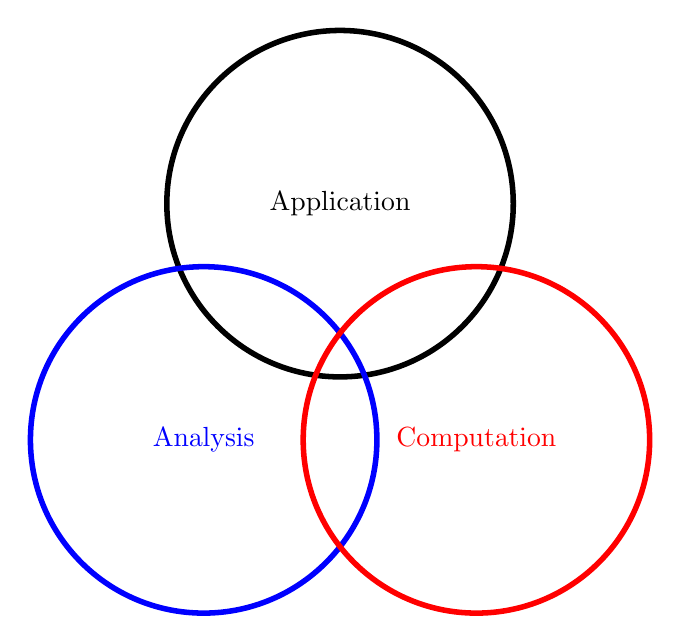
\begin{tikzpicture}
  \draw[black,line width=2pt] (0,2cm) 
    node {Application} circle (2.2 cm);
  \draw[blue,line width=2pt]  (-1.732cm,-1cm) 
    node {Analysis} circle (2.2 cm);
  \draw[red,line width=2pt] ( 1.732cm,-1cm) 
    node {Computation} circle (2.2 cm);
  \end{tikzpicture}
  \end{center}
\end{frame}

\begin{frame}
  \frametitle{Applications Everywhere!}

  These tools are used in more places than you might think:
  \begin{itemize}
  \item Climate modeling
  \item CAD tools (computers, buildings, airplanes, ...)
  \item Control systems
  \item Computational biology
  \item Computational finance
  \item Machine learning and statistical models
  \item Game physics and movie special effects
  \item Medical imaging
  \item Information retrieval
  \item ...
  \end{itemize}
  Parallel computing shows up in all of these.

\end{frame}


\begin{frame}
  \frametitle{Why Parallel Computing?}

  \begin{itemize}
  \item Scientific computing went parallel long ago
    \begin{itemize}
    \item Want an answer that is right enough, fast enough
    \item Either of those might imply a lot of work!
    \item ... and we like to ask for more as machines get bigger
    \item ... and we have a lot of data, too
    \end{itemize}
  \item Today: Hard to get a non-parallel computer!
    \begin{itemize}
    \item {\tt pac} nodes on C4 (early 2012): 16 cores/node
    \item Our nodes on C4 (early 2009): 8 cores/node
    \item My laptop (early 2011): 4 cores + GPU accelerator
    \item iPhone 5 (early 2012): dual core + GPU accelerator 
    \end{itemize}
  \item Running a cluster $\approx$ Amazon account + credit card
    \begin{itemize}
    \item Check out the MIT StarCluster project!
    \end{itemize}
  \end{itemize}

\end{frame}


\begin{frame}
  \frametitle{Lecture Plan}

  Roughly three parts:
  \begin{enumerate}
  \item {\bf Basics:} architecture, parallel concepts, 
    locality and parallelism in scientific codes
  \item {\bf Technology:} OpenMP, MPI, CUDA/OpenCL, UPC, cloud systems,
    profiling tools, computational steering
  \item {\bf Patterns:} Monte Carlo, dense and sparse linear algebra and PDEs,
    graph partitioning and load balancing, fast multipole, fast transforms
  \end{enumerate}
\end{frame}


\begin{frame}
  \frametitle{Goals for the Class}

  You will learn:
  \begin{itemize}
  \item Basic parallel concepts and vocabulary
  \item Several parallel platforms (HW and SW)
  \item Performance analysis and tuning
  \item Some nuts-and-bolts of parallel programming
  \item Patterns for parallel computing in computational science
  \end{itemize}

  \vspace{5mm}
  You might also learn things about
  \begin{itemize}
  \item C and UNIX programming
  \item Software carpentry
  \item Creative debugging (or swearing at broken code)
  \end{itemize}

\end{frame}


\begin{frame}
  \frametitle{Workload}

  CSE usually requires teams with different backgrounds.
  \begin{itemize}
  \item Most class work will be done in small groups (1--3)
  \item Three assigned programming projects (20\% each)
  \item One final project (30\%)
    \begin{itemize}
      \item Should involve some performance analysis
      \item Best projects are attached to interesting applications
      \item Final presentation in lieu of final exam
    \end{itemize}
  \end{itemize}
\end{frame}


\begin{frame}
  \frametitle{Prerequisites}

  You should have:
  \begin{itemize}
  \item Basic familiarity with C programming
    \begin{itemize}
    \item See CS 4411:
      \href{http://www.cs.cornell.edu/courses/cs4410/2010fa/CS4411/slides/intro_to_c/intro_to_c.pdf}{Intro to C} and
      \href{http://www.cs.cornell.edu/courses/cs4410/2010fa/CS4411/slides/intro_to_c/questions/}{practice questions}.
    \item Might want Kernighan-Ritchie if you don't have it already
    \end{itemize}
  \item Basic numerical methods
    \begin{itemize}
    \item See \href{http://www.cs.cornell.edu/~bindel/class/cs3220-s11}{CS 3220}.
    \item Shouldn't panic when I write an ODE or a matrix!
    \end{itemize}
  \item Some engineering or physics is nice, but not required
  \end{itemize}

\end{frame}


\begin{frame}
  \begin{center}
    Questions?
  \end{center}
\end{frame}


\begin{frame}
  \frametitle{How Fast Can We Go?}
  
  Speed records for the Linpack benchmark:
  \begin{center}
  {\small \url{http://www.top500.org}}
  \end{center}

  \vspace{1cm}
  Speed measured in flop/s (floating point ops / second):
  \begin{itemize}
  \item Giga ($10^9$) -- a single core
  \item Tera ($10^{12}$) -- a big machine
  \item Peta ($10^{15}$) -- current top 10 machines (5 in US)
  \item Exa ($10^{18}$) -- favorite of funding agencies
  \end{itemize}
  Current record-holder: China's Tianhe-2 
  \begin{itemize}
  \item 33.9 Petaflop/s (54.9 theoretical peak)
  \item 17.8 MW + cooling
  \end{itemize}

  \vspace{5mm}
  Projection: Exaflop machine around 2018.
\end{frame}


\begin{frame}
  \frametitle{Tianhe-2 environment}
  
  Commodity nodes, custom interconnect:
  \begin{itemize}
  \item
    Nodes consist of Xeon E5-2692 + \textcolor{red}{Xeon Phi accelerators}
  \item
    Intel compilers + Intel math kernel libraries
  \item
    MPICH2 MPI with customized channel
  \item
    Kylin Linux
  \item
    \textcolor{red}{\bf TH Express-2}
  \end{itemize}
\end{frame}


\begin{frame}
  \frametitle{A US Contender}

  \href{http://www.top500.org/system/177556}{Sequoia at LLNL (3 of 500)}
  \begin{itemize}
  \item 20.1 Petaflop/s theoretical peak
  \item 17.2 Petaflop/s Linpack benchmark ($86\%$ peak)
  \item 14.4 Petaflop/s in a bubble-cloud sim
    ($72\%$ peak) \\
    (2013 Gordon Bell prize)
  \item Gordon Bell from 2010 was $30\%$ peak on ORNL Jaguar \\
    (most recent during F11 offering of 5220)
  \item Performance on a more standard code? 
    \begin{itemize}
    \item $10\%$ is probably very good!
    \end{itemize}
  \end{itemize}
\end{frame}


\begin{frame}
  \frametitle{Parallel Performance in Practice}

  So how fast can I make my computation?
  \begin{itemize}
  \item Peak $ > $ Linpack $ > $ Gordon Bell $ > $ Typical
  \item Measuring performance of real applications is hard
    \begin{itemize}
    \item Typically a few bottlenecks slow things down
    \item And figuring out why they slow down can be tricky!
    \end{itemize}
  \item And we {\em really} care about time-to-solution
    \begin{itemize}
    \item Sophisticated methods get answer in fewer flops
    \item ... but may look bad in benchmarks (lower flop rates!)
    \end{itemize}
  \end{itemize}

  \vspace{1cm}
  See also David Bailey's comments:
  \begin{itemize}
  \item \href{http://crd.lbl.gov/~dhbailey/dhbpapers/twelve-ways.pdf}{\small Twelve Ways to Fool the Masses When Giving Performance Results on Parallel Computers} (1991)
  \item \href{http://crd.lbl.gov/~dhbailey/dhbtalks/dhb-12ways.pdf}{\small Twelve Ways to Fool the Masses: Fast Forward to 2011} (2011)
  \end{itemize}
\end{frame}

\begin{frame}
  \frametitle{Quantifying Parallel Performance}
  
  \begin{itemize}
  \item Starting point: good {\em serial} performance
  \item Strong scaling: compare parallel to serial time on the same
    problem instance as a function of number of processors ($p$)
    \begin{align*}
      \mbox{Speedup} &= \frac{\mbox{Serial time}}{\mbox{Parallel time}} \\[2mm]
      \mbox{Efficiency} &= \frac{\mbox{Speedup}}{p}
    \end{align*}
  \item
    Ideally, speedup = $p$.  
    Usually, speedup $ < p$.
  \item Barriers to perfect speedup
    \begin{itemize}
    \item Serial work (Amdahl's law)
    \item Parallel overheads (communication, synchronization)
    \end{itemize}
  \end{itemize}
\end{frame}

\begin{frame}
  \frametitle{Amdahl's Law}

  Parallel scaling study where some serial code remains:
  \begin{align*}
    p = & \mbox{ number of processors} \\
    s = & \mbox{ fraction of work that is serial} \\
    t_s = & \mbox{ serial time} \\
    t_p = & \mbox{ parallel time} \geq s t_s + (1-s) t_s / p
  \end{align*}

  \vspace{2mm}
  Amdahl's law:
  \[
    \mbox{Speedup} = 
      \frac{t_s}{t_p} = \frac{1}{s + (1-s) / p} > \frac{1}{s}
  \]

  \vspace{5mm}
  So $1\%$ serial work $\implies$ max speedup < $100 \times$,
  regardless of $p$.
\end{frame}

\begin{frame}
  \frametitle{A Little Experiment}
  
  Let's try a simple parallel attendance count:
  \begin{itemize}
  \item {\bf Parallel computation:} Rightmost person in each row 
    counts number in row.
  \item {\bf Synchronization:} Raise your hand when you have a count
  \item {\bf Communication:} When all hands are raised, each row 
        representative adds their count to a tally and says the sum
        (going front to back).
  \end{itemize}

  \vspace{5mm}
  (Somebody please time this.)

\end{frame}


\begin{frame}
  \frametitle{A Toy Analysis}

  Parameters:
  \begin{align*}
    n = & \mbox{ number of students} \\
    r = & \mbox{ number of rows} \\
    t_c = & \mbox{ time to count one student} \\
    t_t = & \mbox{ time to say tally} \\
    t_s \approx & ~n t_c \\
    t_p \approx & ~n t_c / r + r t_t
  \end{align*}

  \vspace{5mm}
  How much could I possibly speed up?

\end{frame}


\begin{frame}
\frametitle{Modeling Speedup}

\begin{center}
  \begin{tikzpicture}
  \begin{axis}[
    width = {\textwidth},
    height = {0.6\textheight},
    xlabel = {Rows},
    ylabel = {Predicted speedup}]
  \addplot file {lec01plot.dat};
  \end{axis}
  \end{tikzpicture} \\[1cm]
(Parameters: $n = 80$, $t_c = 0.3$, $t_t = 1$.)
\end{center}
\end{frame}


\begin{frame}
\frametitle{Modeling Speedup}

The bound
\[
  \mathrm{speedup} < 
  \frac{1}{2} \sqrt{\frac{n t_c}{t_t}} 
\]
is usually tight.
\vspace{5mm}

Poor speed-up occurs because:
\begin{itemize}
\item The problem size $n$ is small
\item The communication cost is relatively large
\item The serial computation cost is relatively large
\end{itemize}
Some of the usual suspects for parallel performance problems! \\[5mm]
Things would look better if I allowed both $n$ and $r$ to grow ---
that would be a {\em weak} scaling study.

\end{frame}

\begin{frame}
  \frametitle{Summary: Thinking about Parallel Performance}

  Today:
  \begin{itemize}
  \item We're approaching machines with peak {\em exaflop} rates
  \item But codes rarely get peak performance
  \item Better comparison: tuned serial performance
  \item Common measures: {\em speedup} and {\em efficiency}
  \item Strong scaling: study speedup with increasing $p$
  \item Weak scaling: increase both $p$ and $n$
  \item Serial overheads and communication costs kill speedup
  \item Simple analytical models help us understand scaling
  \end{itemize}

  \vspace{5mm}
  Next week: Getting started on C4 + basic architecture and serial performance.
\end{frame}

\begin{frame}
  \frametitle{And in case you arrived late}

  \begin{center}
  {\small \url{http://www.cs.cornell.edu/~bindel/class/cs5220-s14/}} \\
  {\small \url{https://bitbucket.org/dbindel/cs5220-s14/wiki/Home}} \\
  {\small \url{http://www.piazza.com/cornell/spring2014/cs5220}}
  \\[1cm]
  ... and send me your netid if not enrolled!
  \end{center}

\end{frame}

\end{document}
